\documentclass[a4paper,12pt]{article}

\usepackage[slovene]{babel}
\usepackage{amsfonts,amssymb,amsmath}
\usepackage[utf8]{inputenc}
\usepackage[T1]{fontenc}
\usepackage{lmodern}
\usepackage{graphicx}

\def\qed{$\hfill\Box$}   % konec dokaza
\def\qedm{\qquad\Box}   % konec dokaza v matematičnem načinu
\newtheorem{izrek}{Izrek}
\newtheorem{trditev}{Trditev}
\newtheorem{posledica}{Posledica}
\newtheorem{lema}{Lema}
\newtheorem{opomba}{Opomba}
\newtheorem{definicija}{Definicija}
\newtheorem{zgled}{Zgled}

\title{Kromatično število Kneserjevih grafov \\ 
\Large Seminar}
\author{Žan Hafner Petrovski \\
Fakulteta za matematiko in fiziko \\
Oddelek za matematiko}
\date{12.\ maj 2017}

\begin{document}

%%%%
 
\maketitle
\newpage

%%%%

\section{Uvod}

V teoriji grafov poznamo mnogo različnih tipov grafov. Razlikujemo jih glede na njihove specifične lastnosti. V tem seminarju se bomo ukvarjali s {\em Kneserjevimi grafi} oziroma podrobneje, s {\em kromatičnim številom} le-teh. Najprej podajmo nekaj glavnih definicij.

%%%%

\begin{definicija}
Graf $K(n,k)$, $n \geq k \geq 1$ in $n, k \in \mathbb{N}$, imenujemo \mbox{\textbf{Kneserjev}}, če je množica vozlišč $V(n,k)$ družina vseh $k$-elementnih podmnožic množice $\{1, 2, \ldots, n\}$. Dve vozlišči sta povezani natanko takrat, ko sta disjunktni. 
\end{definicija}

Povejmo še, da za število vozlišč velja $|V(n,k)|={{n}\choose{k}}$. V primeru, ko je $n < 2k$, imata vsaki dve $k$-elementni množici neprazen presek. Tak Kneserjev graf nima nobenih povezav, zato privzemimo, da velja $n \geq 2k$.


\begin{definicija}
Najmanjše število $m$, ki zadošča barvanju vozlišč grafa $G$, imenujemo \textbf {Kromatično število}. Označimo ga s $\chi(K(n,k)).$
\end{definicija}

\begin{definicija}
Preslikavo $c: V \rightarrow \{1, \ldots, m\}$, ki slika vozlišča grafa v množico barv, imenujemo \textbf {barvanje}. Ta preslikava zadošča pogoju, da sta vsaki dve sosednji vozlišči pobarvani z različnima barvama.
\end{definicija}

Kromatično število grafa $G$ je torej najmanjše število barv, s katerimi lahko pobarvamo vozlišča grafa tako, da se nobeni dve sosednji vozlišči ne slikata v isto barvo. Množico vozlišč $V$ bi radi predstavili kot disjunktno unijo barvnih razredov $V = V_1 \sqcup V_2 \sqcup \ldots \sqcup V_{\chi(G)}$, teh pa želimo, da je najmanj. 



Za vsak barvni razred velja, da imajo vsi njegovi elementi, torej $k$-elementne množice, neprazen presek. To sledi iz definicije Kneserjevih grafov, če bi imele te množice prazen presek, to je, obstajali bi vsaj dve disjunktni, med katerima bi obsatjala povezava, zato pa bi bili pobarvani z različno barvo.

Vozlišča Kneserjevega grafa $K(n,k)$ bomo razdelili na disjunktne množice $V = V_1 \sqcup V_2 \sqcup \ldots \sqcup V_{\chi(K(n,k))}$, kjer bo vsak $V_i$ družina množic moči $k$ z nepraznim presekom. Ker smo predpostavili, da je $n \geq 2k$, poenostavimo zapis in pišimo $n = 2k + d, k \geq 1, d \geq 0$.

\newpage
\begin{zgled}{Kneserjev graf $K(5,2)$ je zelo znan primer, imenujemo ga Petersenov graf. 

\begin{figure}[h!]
	\centering
	\begin{minipage}{0.45\textwidth}
		\centering
		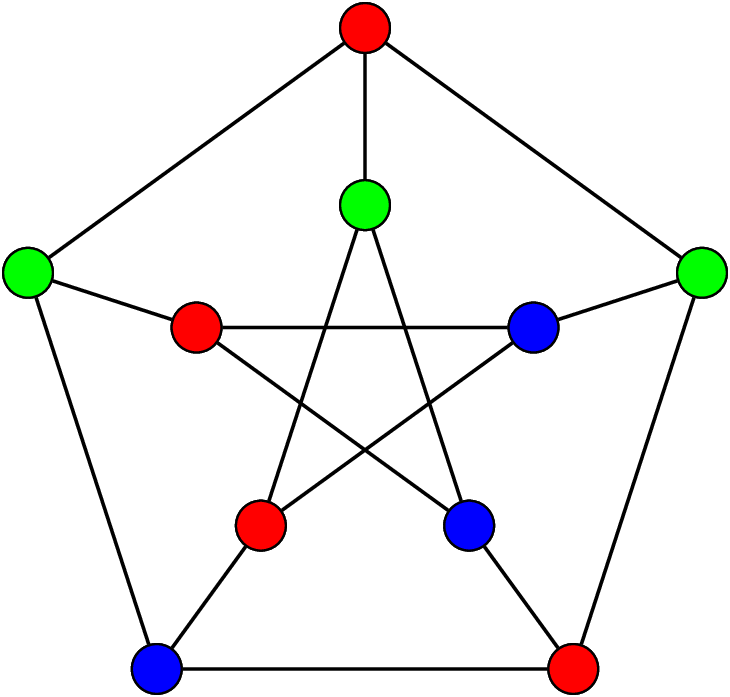
\includegraphics[width=0.8\textwidth]{petersenov_graf_barvanje} % first figure itself
        	\caption{Primer barvanja tega grafa z $d+2$, torej $3$ barvami}
    	\end{minipage}\hfill
    	\begin{minipage}{0.45\textwidth}
       	 \centering
        	 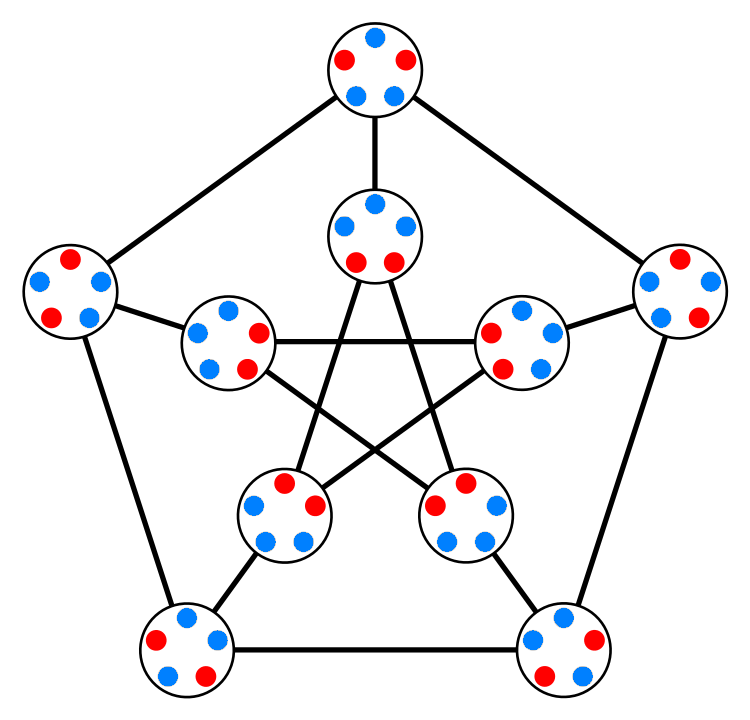
\includegraphics[width=0.8\textwidth]{petersenov_graf_mnozice} % second figure itself
       	 \caption{Prikaz povezav med disjunktnimi množicami}
    	\end{minipage}
\end{figure}
}

\end{zgled}

Da dobimo idejo, s koliko barvami zanesljivo lahko pobarvamo Kneserjev graf, zapišimo preprost predpis za barvanje grafa $K(2k+d,k)$, pri katerem uporabimo $d+2$ barv. Za števila i iz $\{1,2,\ldots,d+1\}$ naj množica $V_i$ sestoji iz vseh $k$-elementnih množic, ki imajo $i$ za najmanjši element. Preostale \mbox{$k$-elementne} množice so vsebovane v množici $\{d+2,d+3,\ldots,2k+d\}$, katere moč je le $2k-1$. Sledi, da imajo te množice neprazen presek in lahko zanje uporabimo barvo $d+2$. 

Tako smo dobili $\chi(K(2k+d,k)) \leq d+2$. Kneser je postavil domnevo, da je $d+2$ kar najmanjše možno število barv, torej kromatično število Kneserjevega grafa $K(2k+d,k)$.

\section{Kneserjeva domneva}

Cilj tega seminarja je dokazati naslednji izrek:
\begin{izrek}[Kneser]
Za kromatično število Kneserjevega grafa velja
$$\chi(K(2k+d,k)) = d+2.$$
\end{izrek}

\noindent
Preformulirajmo ta izrek v obliko problema obstoja na sledeč način:

\begin{izrek}[Ekvivalenten Kneserjevemu izreku]
Če družino $k$-elementnih podmnožic množice $\{1, 2, \ldots, 2k+d\}$ razdelimo na $d+1$ razredov,  $V = V_1 \sqcup V_2 \sqcup \ldots \sqcup V_{d+1}$, potem obstaja $i$, da $V_i$ vsebuje par $k$-elementnih disjunktnih množic $A$ in $B$.
\end{izrek}

Tako smo prišli do splošnejše različice izreka. Ta nam, še preden se poglobimo v sam dokaz, nudi drugačen pogled na zastavljen problem, saj ne omenja grafov. Želimo le pokazati obstoj množic $A$ in $B$. László Lovász je uvidel, da bistvo problema tiči v slavnem izreku o $d$-dimenzionalni enotski sferi $S^d$ v $\mathbb{R}^d $, $S^d = \{x \in \mathbb{R}: |x|=1\}$. Zapišimo še ta izrek.

\begin{izrek}[Borsuk-Ulam]
Za vsako zvezno preslikavo $f:S^d \rightarrow \mathbb{R}^d$, z $d$-sfere v $d$-prostor, obstajata antipodni točki $x^*$ in $-x^*$, ki ju $f$ slika v isto točko, torej $f(x^*)=f(-x^*)$.
\end{izrek}

Dokaz tega izreka lahko bralec najde v knjigi ''Using the Borsuk-Ulam theorem'' matematika Jirija Matouška, mi pa se bomo posvetili njegovi uporabi pri dokazu izreka Lyusternika in Shnirel'mana.

\begin{izrek}[Lyusternik-Shnirel'man]
Če je $d$-sfera $S^d$ pokrita z $d+1$ množicami,
$$S^d = U_1 \cup U_2 \cup \ldots \cup U_d \cup U_{d+1},$$
tako, da so vse izmed prvih $d$ množic $U_1, U_2, \ldots, U_d$ bodisi odprte bodisi zaprte, potem ena izmed $d+1$ množic vsebuje par antipodnih točk $x^*$ in $-x^*$.
\end{izrek}

\noindent
{\em Dokaz s protislovjem in uporabo Borsuk-Ulamovega izreka:} \\
\indent Naj bo pokritje $S^d = U_1 \cup U_2 \cup \ldots \cup U_d \cup U_{d+1}$ dano, kot je zapisano v izreku. Predpostavimo, da noben izmed $U_i$ ne vsebuje dveh antipodnih točk. Definirajmo preslikavo $f:S^d \rightarrow \mathbb{R}^d$ na sledeč način:
$$f(x) := (d(x,U_1), d(x,U_2), \ldots, d(x,U_d)).$$
Tu $d(x,U_i)$ označuje razdaljo med točko $x$ in množico $U_i$. \\
\indent Ker je to zvezna funkcija na $x$, je tudi $f$ zvezna. Torej lahko uporabimo Borsuk-Ulamov izrek, ki nam pove, da na domeni $f$, torej na $S^d$, obstajata antipodni točki $x^*$ in $-x^*$ z lastnostjo $f(x^*)=f(-x^*)$. Ker po predpostavki z začetka dokaza $U_{d+1}$ ne vsebuje antipodnih točk, sklepamo, da je vsaj en izmed $x^*$ in $-x^*$ vsebovan v eni izmed množic $U_i$, recimo v $U_k$ za $k\leq d$. Brez škode za splošnost lahko privzamemo, da je to $x^*$, torej $x^* \in U_k$. To pomeni, da je $d(x^*, U_k) = 0$, ključno pa je, da je zaradi lastnosti $f(x^*)=f(-x^*)$ tudi $d(-x^*, U_k) = 0$.\\
\indent Obravnavajmo najprej primer, ko je $U_k$ zaprt. Potem iz $d(-x^*, U_k) = 0$ sledi, da je $-x^* \in U_k$, kar pa je protislovje s predpostavko, da noben izmed $U_i$ ne vsebuje para antipodnih točk.\\
\indent Če je $U_k$ odprt, potem iz $d(-x^*, U_k) = 0$ sledi, da $-x^*$ leži v zaprtju $U_k$, torej v $\overline U_k$. Ta množica pa je vsebovana v $S^d\textbackslash(-U_k)$, \mbox{$-U_k = \{-x;x \in U_k\}$}. Množica $S^d\textbackslash(-U_k)$ je namreč zaprta in vsebuje $U_k$, pri tem smo upoštevali predpostavko, da $U_k$ ne vsebuje antipodnih točk. Ampak, ker je zaprta in vsebuje $U_k$, vsebuje tudi $\overline U_k$. To pomeni, da $-x^*$ leži v  $S^d\textbackslash(-U_k)$, torej ne more ležati v $-U_k$. Ker pa smo privzeli, da $x^* \in U_k$, smo prišli do protislovja. \qed

V svojem dokazu iz leta 1978 je Imre Bárány uporabil še Galeov izrek o obstoju določene postavitve točk na sfero $S^d$. Bárány je svoj dokaz objavil nekaj tednov za tem, ko je László Lovász prvi dokazal Kneserjevo domnevo s pomočjo Borsuk-Ulamovega dokaza.

\begin{izrek}[Gale]
Obstaja taka postavitev $2k+d$ točk na $d$-dimenzionalno sfero $S^d$, da vsaka odprta polsfera vsebuje vsaj $k$ izmed teh točk.
\end{izrek}

Leta 2002 je dodiplomski študent Joshua Greene nadalje poenostavil Bárányjev dokaz. Ugotovil je namreč, da zadošča, če so točke iz izreka v splošni legi na sferi. Tu je zapisan Greeneov dokaz.

\begin{definicija}
Točke iz množice $\{1,2,\ldots,2k+d\}$ so v \textbf {splošni legi} na sferi $S^{d+1}$, če nobenih $d+2$ točk iz omenjene množice ne leži na hiperravnini skozi središče sfere.
\end{definicija}

\noindent
{\em Dokaz Kneserjeve domneve:}

\indent Vzemimo množico $2k+d$ točk v splošni legi na sferi $S^{d+1}$. Naj bo $V(n,k)$ množica vseh $k$-elementnih podmnožic začetne množice, razdelimo jo na $d+1$ razredov, $V(n,k) = V_1 \sqcup V_2 \sqcup \ldots \sqcup V_{d+1}$. Naš cilj je najti par disjunktnih $k$-elementnih množic $A$ in $B$, ki pripadata istemu razredu $V_i$.

Za $i=1, 2,\ldots, d+1$ definirajmo
\begin{align*} O_i = \{x \in S^{d+1}; &\text{ odprta polsfera } H_x \text{ z vrhom } x \\ &\text{ vsebuje } k\text{-elementno množico iz } V_i\}.
\end{align*}

\begin{figure}[h!]
\centering
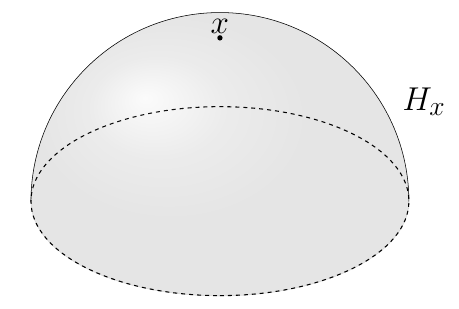
\includegraphics[width=0.4\textwidth]{polsfera}
\end{figure}

Vsaka množica $O_i$ je odprta. Za vsak $x \in O_i$ namreč obstaja neka odprta okolica, za vsak element $y$ iz te okolice pa še vedno velja, da polsfera, katere vrh je $y$, vsebuje istih $k$-elementov kot polsfera, katere vrh je $x$. To sledi iz dejstva, da smo v definiciji množic $O_i$ uporabili {\em odprte} polsfere.

Odprte množice $O_i$ in zaprta množica $C = S^{d+1} \backslash (O_1 \cup \ldots \cup O_{d+1})$ tvorijo pokritje $S^{d+1}$. To pokritje zadošča pogoju iz izreka Lyusternik-Shnirel'mana, zato vemo, da ena izmed množic iz omenjenega pokritja vsebuje antipodni točki $x^*$ in $-x^*$. 

To ne more biti množica $C$, saj po definiciji množic $O_i$ polsferi $H_{x^*}$ in $H_{-x^*}$, ko velja $x^*, -x^* \in C$, vsebujeta manj kot $k$ točk. To je res, saj unija množic $O_i$ vsebuje {\em vse} $k$-elementne podmnožice začetne množice, $C$ pa je komplement te unije. Sledi, da vsaj $d+2$ točki ležita na ekvatorju $\overline H_{x^*} \cap \overline H_{-x^*}$, torej na hiperravnini skozi središče sfere. To pa ne more biti res, saj so točke v splošni legi.

Zato ena izmed množic $O_i$ vsebuje antipodni točk $x^*$ in $-x^*$. Po definiciji množic $O_i$  obstajata \mbox{$k$-elementni} množici $A, B \in V_i$ z lastnostjo $A \subseteq H_{x^*}$ in $B \subseteq H_{-x^*}$. 

Ker pa govorimo o {\em odprtih} polsferah, sta $H_{x^*}$ in $H_{-x^*}$ disjunktni. Sledi, da sta tudi $A$ in $B$ disjunktni. Našli smo torej $k$-elementni množici, ki pripadata istemu razredu množic $V_i$. \qed


%%%%

\begin{thebibliography}{1}

\bibitem{AiZ}
M.~Aigner in G.~M.~Ziegler, \emph{Proofs from THE BOOK}, 2.\ izdaja, Springer, Berlin--Heidelberg--New York, 2001.
%https://math.berkeley.edu/{tu manjka ~}brandtm/research/kneser.pdf (25.4.2017)
%http://oai.cwi.nl/oai/asset/9898/9898A.pdf

%slike
%https://graphtheoryinlatex.files.wordpress.com/2010/02/coloringpeteresen2.png
%http://blogs.ams.org/visualinsight/files/2015/06/petersen_graph.png
\end{thebibliography}

\end{document}